% ============================================================================
% Fragment-Causal Storage as a Common Substrate: the sfs artifact
% arXiv preprint skeleton
% ============================================================================
\documentclass[a4paper, 11pt, twoside]{article}

% ── Encoding & language ────────────────────────────────────────────────────
\usepackage[utf8]{inputenc}
\usepackage[T1]{fontenc}
\usepackage[english]{babel}
\usepackage{csquotes}

% ── Fonts ──────────────────────────────────────────────────────────────────
\usepackage{lmodern}
\usepackage{microtype}

% ── Page layout ─────────────────────────────────────────────────────────────
\usepackage[
  top=2.5cm,
  bottom=2.5cm,
  left=2.8cm,
  right=2.8cm,
]{geometry}

% ── Math (light — this is a systems paper) ─────────────────────────────────
\usepackage{amsmath}
\usepackage{amssymb}

% ── Graphics, tables, code, algorithms ─────────────────────────────────────
\usepackage{graphicx}
\usepackage{booktabs}
\usepackage{multirow}
\usepackage{subcaption}
\usepackage{tikz}
\usetikzlibrary{positioning, arrows.meta, fit, backgrounds}
\usepackage{pgfplots}
\pgfplotsset{compat=1.18}
\usepackage{enumitem}
\usepackage{listings}
\usepackage{algorithm}
\usepackage{algorithmic}

% ── Code listing style ──────────────────────────────────────────────────────
\lstset{
  basicstyle=\ttfamily\small,
  columns=fullflexible,
  keepspaces=true,
  breaklines=true,
  frame=none,
}

% ── Colors & hyperref ──────────────────────────────────────────────────────
\usepackage[dvipsnames, svgnames]{xcolor}
\usepackage[
  colorlinks=true,
  linkcolor=NavyBlue,
  citecolor=ForestGreen,
  urlcolor=RoyalBlue,
]{hyperref}
\usepackage[nameinlink, capitalise, noabbrev]{cleveref}

% ── Bibliography ────────────────────────────────────────────────────────────
\usepackage[numbers, sort&compress]{natbib}
\bibliographystyle{plainnat}

% ── Convenience macros ──────────────────────────────────────────────────────
\newcommand{\sfs}{\textsc{sfs}}
\newcommand{\eg}{e.g.,\ }
\newcommand{\ie}{i.e.,\ }

% ── Document metadata ───────────────────────────────────────────────────────
\title{\textsc{sfs}: A Fragment-Causal Filesystem Substrate for Agentic Time\\
  across Machines, Encrypted SaaS, and WebAssembly}

\author{%
  Sandra Theresa Ke\ss{}ler\thanks{%
    Independent researcher. Correspondence:
    \texttt{mail@sandra-kessler.net}.}%
}

\date{July 2026}

% ============================================================================
\begin{document}
% ============================================================================

\maketitle

\begin{abstract}
Parallel software agents increasingly edit one body of files from different
processes and machines.  They need Git-like retained history and conflict
visibility, but synchronization must be continuous rather than organized around
explicit repository commits.  Versioning, synchronization, encrypted remote
storage, and portable execution are commonly separate layers whose boundaries
give one update several identities: a filesystem block, a version-control
delta, a synchronization object, and a cloud object.  We present \sfs{}, a
filesystem substrate motivated by this \emph{agentic-time} setting that instead
makes a position-addressed \emph{fragment version map} the common
representation.  Each unit carries a
sparse version vector and, for every fragment position, the causal dot of the
bytes currently selected there.  The map is simultaneously a retained local
lineage, a synchronization manifest, and the basis for sub-file conflict
classification.  Concurrent updates to disjoint fragments merge without a
content-specific CRDT.  Concurrent updates to the same fragment remain visible
as separate strains.

Around this representation, \sfs{} combines deterministic fixed-size chunking,
atomic root publication, retained versions and named cuts, client-side-encrypted
synchronization, and an epoch-versioned multi-writer authorization model.  The
same synchronization protocol operates against either a blind cloud store or a
live peer.  In the secure deployment profile, content and metadata are
client-side AES-GCM encrypted and accepted record frontiers are authorized by
an owner-signed writer set.  The service receives neither plaintext nor the keys
needed to derive it.  A single v12 container format is implemented by a
memory-safe Rust core, a FUSE adapter over host-file containers, an independent
in-kernel C driver over raw devices, a C ABI, and experimental in-memory
WebAssembly bindings.  The same logical state therefore crosses an execution
boundary (kernel/userspace/browser) and a trust boundary (local media/encrypted
service) without conversion into a second storage model.

Deterministic multi-replica scenarios exercise disjoint-fragment convergence,
same-fragment strain preservation and resolution, third-replica discovery, and
bidirectional synchronization with a live TLS peer.  They establish the
mechanisms in small controlled topologies, not behavior at agent-fleet scale.
We separately evaluate the mounted Linux paths over 14 I/O sizes using ten
fault-checked runs per cell.  Under the reported single-threaded protocol,
kernel-path geometric means are $1.22\times$ ext4 for plaintext writes,
$0.98\times$ for plaintext cold reads, $0.98$--$0.99\times$ ext4-on-LUKS for
encrypted writes,
and $1.11$--$1.20\times$ for encrypted cold reads.  The FUSE path reaches
$3.11\times$ \texttt{fuse2fs} for plaintext writes and $1.70\times$ for
plaintext cold reads, but only $0.33$--$0.38\times$ \texttt{gocryptfs} for
encrypted cold reads.  These results establish a competitive native path and
identify the userspace encrypted-read path as the principal performance limit.
They do not constitute a general workload or scalability evaluation.  As a
secondary result, an annex reports a NoSQL projection built without changing
the core representation.
\end{abstract}


\section{Introduction}
\label{sec:intro}

The motivating question for \sfs{} is simple: what should a filesystem look
like when many software agents edit one project concurrently across machine
boundaries?  Git provides durable history, branching, and explicit merge, but
its repository and commit model sits above the live filesystem.  File
synchronizers propagate live state, but commonly reduce a concurrent edit to a
whole-file conflict.  An \emph{agentic-time filesystem} should make history and
causality intrinsic, synchronize continuously, preserve rather than overwrite
unresolved alternatives, and still present ordinary files to tools that know
nothing about the replication protocol.

The immediate design prompt came from Theo Browne's 2026 discussion of source
control, filesystems, and a ``Dropbox for devs''~\citep{Browne2026Ideas}.  The
segment asks for one code-tree structure across local machines and cloud
agents, with content materialized when a participant touches it rather than
through manual clone and worktree choreography.  \sfs{} takes that prompt as a
filesystem problem, then adds the properties needed for concurrent autonomous
writers: retained causal history, fragment-level conflict visibility, client-
side encryption, and signed writer authorization.  We use \emph{agentic time}
for this resulting workload, not as a claim that the later mechanisms appeared
in the original prompt.

Local storage abstractions are usually divided by execution and trust boundary.
A kernel filesystem owns raw media and POSIX semantics; a portable userspace
filesystem places a container on another filesystem; a browser uses an
in-memory or origin-private backend; and cloud synchronization converts local
state into provider objects.  Snapshots or a version-control system add
history, while an encrypting layer protects the remote copy.  The resulting
stack works, but the boundaries duplicate identity, causality, indexing, and
recovery state.

This mismatch matters for local-first workloads~\citep{Kleppmann2019LocalFirst}
in which the same state is edited on several machines, may be stored by a
provider that should not see its contents, and is consumed through more than
one execution environment.  Agentic development is the primary workload:
small, frequent, partly overlapping changes from independent actors must remain
recoverable and synchronizable without forcing each agent to coordinate an
explicit commit.  The architecture also applies to financial, collaborative,
or personal-data applications whose virtual filesystem is useful only when its
bytes remain client-side encrypted and writer-authorized from browser or native
client through persistence and synchronization.  The service should transport
and retain state without ever receiving the content or metadata key.

Prior systems cover large parts of this space.  Versioning filesystems retain
past states~\citep{Santry1999Elephant,Soules2003CVFS,Peterson2005Ext3cow}; Coda,
Ficus, and Ivy support optimistic replication~\citep{Kistler1992Coda,
Reiher1994Ficus,Muthitacharoen2002Ivy}; Plutus, SiRiUS, SUNDR, and SPORC address
sharing over untrusted storage under different threat
models~\citep{Kallahalla2003Plutus,Goh2003SiRiUS,Li2004SUNDR,Feldman2010SPORC};
and WNFS and Peergos combine encrypted, portable, collaborative
storage~\citep{WNFSspec,Peergos}.  Ceph demonstrates one distributed object
substrate behind file, block, and object interfaces~\citep{Weil2006Ceph}.
Consequently, our claim is not that any one capability, nor the general idea of
multiple surfaces over one substrate, is new.

\sfs{} explores a narrower systems question: \emph{what follows if a
position-addressed fragment version map is the common state representation
across execution and trust boundaries?}  A unit has a stable UUID, a sparse
version vector, and an ordered map from fragment position to the causal dot of
the selected bytes.  A write replaces only the affected positions.  The same
map then provides four functions:

\begin{enumerate}[leftmargin=1.6em,itemsep=2pt]
  \item it is the materialized current version and the index into retained
    fragment history;
  \item it is the manifest used to identify missing or changed synchronization
    payloads;
  \item together with the version vector, it classifies concurrent updates per
    fragment, automatically merging disjoint changes and preserving overlapping
    ones as strains; and
  \item its logical identity is independent of physical location and backend,
    allowing the same container semantics in a raw-device kernel VFS, a
    userspace host-file VFS, an in-memory WebAssembly adapter, and an encrypted
    remote transport.
\end{enumerate}

Several supporting choices make this representation usable as a filesystem and
application VFS.  Deterministic fixed-size fragments give constant-time
offset-to-fragment addressing within a geometry band.  A double-buffered
authenticated header is the atomic publication point, while an optional
write-ahead log and bounded undo records cover asynchronous and in-place paths.
Metadata is always protected by AES-GCM; content is selectable per fragment as
GCM, XTS, or plaintext.  The secure application profile selects GCM content and
an owner-signed writer set.  In that profile the service receives no content
key, path, metadata plaintext, or content plaintext.  Account, object,
version-vector, size, timing, and access-pattern metadata remain visible.
Per-record Ed25519 signatures and the writer set authorize multi-writer record
frontiers.  These mechanisms are described in \cref{sec:design}.

The design is implemented rather than simulated.  A
\texttt{\#![forbid(unsafe\_code)]} Rust core, a FUSE adapter, and an independent
in-kernel C driver read and write the current v12 format.  The same engine is
also exposed through a C ABI and experimental in-memory WebAssembly bindings.
Synchronization runs unchanged against a blind service or a live peer
implementing the same transport contract.  Controlled functional scenarios
follow convergence through two and three replicas, hosted TLS, and a live peer.
The performance study separately compares the raw-device kernel path and the
container-on-ext4 FUSE path only with matching stacks (\cref{sec:eval}).

\paragraph{Contributions.}
\begin{itemize}[leftmargin=1.4em,itemsep=2pt]
  \item \textbf{A fragment-causal storage representation} in which the ordered
    fragment map and sparse version vector jointly serve local history,
    synchronization, and sub-file conflict classification
    (\cref{subsec:mvcc,subsec:sync}).
  \item \textbf{Execution- and topology-independent storage}: one v12 logical
    format is implemented by a raw-device kernel VFS, a userspace host-file VFS,
    the Rust engine and C ABI, and experimental in-memory WebAssembly bindings;
    one synchronization protocol operates against either a blind multi-tenant
    service or another live container, including propagation of concurrent
    frontiers, writer sets, and epoch-tagged key grants
    (\cref{subsec:transport,sec:impl}).
  \item \textbf{An atomic-publication, recovery, and allocation design}
    (\cref{subsec:commit,subsec:alloc}): a double-buffered, sequence-wins header
    commit plus fragment-granular copy-on-write and bounded undo records over a
    flat three-region allocator.  An optional WAL serves the asynchronous write
    path.  File content avoids recursive path shadowing in a global CoW tree;
    the catalog tries retain their own CoW cost.
  \item \textbf{A controlled artifact evaluation}
    (\cref{sec:impl,sec:eval}): deterministic multi-replica scenarios for
    merge, retained conflict, resolution, hosted sync, and live-peer sync, plus
    a fault-aware Linux throughput study that reports both the competitive
    native path and the remaining encrypted FUSE-read deficit.
\end{itemize}

A document/KV projection is included as an annex
(\cref{sec:annex-nosql}) rather than a primary
contribution.  It is useful evidence that the unit abstraction is not tied to
POSIX paths, but the paper's subject is the backend and its VFS, SaaS, peer, and
WebAssembly boundaries.

\Cref{sec:background} defines the representation and positions the design;
\cref{sec:design} gives its mechanisms and invariants; \cref{sec:impl,sec:eval}
describe the artifact and evaluation; and \cref{sec:related,sec:discussion}
separate the contribution from related systems and state its limits.


\section{Background and the Capability Gap}
\label{sec:background}

\subsection{One Update, Several Representations}

Consider two replicas that start from the same file.  Replica A changes bytes
in one region and replica B changes another.  A conventional local filesystem
records two unrelated block updates.  A file-level synchronizer sees two
concurrent file versions and must either select one or ask a content-specific
merger.  Encryption and remote storage add further mappings between logical
content, local physical blocks, and opaque provider objects.

\sfs{} preserves causal structure below every surface and separates logical
fragment identity from its physical backend and cipher encoding.  The basic
state of a content stream is

\begin{equation}
  U = (\mathit{uuid}, e, \ell, VV, M), \qquad
  M[f] = d_f = (a_f,c_f),
\end{equation}

where $e$ is the fragment-size exponent, $\ell$ the logical length of the last
fragment, $VV$ a sparse version vector, and $M$ an ordered map from fragment
index $f$ to a causal dot containing replica alias $a_f$ and counter $c_f$.
This tuple is the replica-invariant logical head, not the complete physical
record.  A materialized record additionally contains selected locations and a
parent address used to walk local retained lineage.  Parent is omitted from
$U$ because replicas may store the same logical head at different addresses
and construct different physical parent chains during import, relocation, or
re-ciphering.  It is consequently excluded from logical record signatures and
transport identity.  Physical locations and cipher encodings are omitted for
the same reason: they may change without creating a new logical version.

This model separates three granularities that are often conflated.  A
byte-range is the API granularity of a read or write.  A fragment is the unit of
storage, transfer, and merge classification.  A unit is the scope of the
version vector and user-visible conflict.  Consequently, \sfs{} provides
byte-addressed I/O but fragment-granular causality.

\subsection{Design Requirements}

The representation is useful only if it satisfies the surrounding systems
requirements.  First, reconstructing the current unit must not replay its
history: the head map and selected fragments are materialized.  Second,
publication of a new map and catalog roots must be atomic.  Third, a sync pass
must transfer changed or missing fragments while retaining all concurrent
frontiers.  Fourth, the transport must not need content keys or plaintext.
Fifth, physical encoding and execution surface must be separable from logical
identity so that kernel, userspace, embedded, and browser-facing adapters can
share the format.

These requirements are not individually new.  \Cref{tab:positioning} therefore
positions representative systems by their architectural center rather than by
a checklist constructed around \sfs{}.

\begin{figure}[t]
  \centering
  \resizebox{\linewidth}{!}{%
  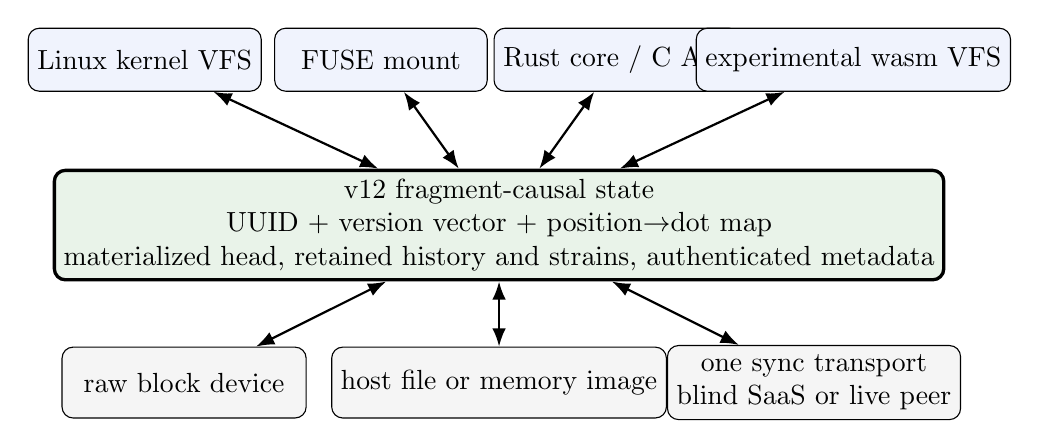
\begin{tikzpicture}[
    surface/.style={draw, rounded corners, align=center, minimum width=2.7cm,
                    minimum height=0.8cm, fill=RoyalBlue!8},
    core/.style={draw, rounded corners, align=center, minimum width=8.8cm,
                 minimum height=1.25cm, fill=ForestGreen!10, very thick},
    backend/.style={draw, rounded corners, align=center, minimum width=3.1cm,
                    minimum height=0.9cm, fill=black!4},
    link/.style={<->, >=Latex, thick}]
    \node[surface] (kernel) at (-4.5,2.1) {Linux kernel VFS};
    \node[surface] (fuse)   at (-1.5,2.1) {FUSE mount};
    \node[surface] (api)    at ( 1.5,2.1) {Rust core / C ABI};
    \node[surface] (wasm)   at ( 4.5,2.1) {experimental wasm VFS};

    \node[core] (state) at (0,0)
      {v12 fragment-causal state\\
       UUID + version vector + position$\rightarrow$dot map\\
       materialized head, retained history and strains, authenticated metadata};

    \node[backend] (raw)  at (-4.0,-2.0) {raw block device};
    \node[backend] (file) at ( 0.0,-2.0) {host file or memory image};
    \node[backend] (sync) at ( 4.0,-2.0) {one sync transport\\blind SaaS or live peer};

    \draw[link] (kernel) -- (state);
    \draw[link] (fuse) -- (state);
    \draw[link] (api) -- (state);
    \draw[link] (wasm) -- (state);
    \draw[link] (state) -- (raw);
    \draw[link] (state) -- (file);
    \draw[link] (state) -- (sync);
  \end{tikzpicture}%
  }
  \caption{One logical representation crosses execution boundaries above and
  physical or trust boundaries below.  The hosted service stores protocol
  objects rather than interpreting filesystem operations.}
  \label{fig:architecture}
\end{figure}

\Cref{fig:architecture} is the paper's organizing distinction.  The surfaces
do not create their own version models, and the hosted path does not introduce
a server-authoritative namespace.  They adapt one logical state to different
execution and persistence boundaries.

\begin{table}[t]
  \centering
  \small
  \setlength{\tabcolsep}{4pt}
  \caption{Architectural centers of representative neighboring systems.  The
    rows are not an ordering: several systems provide stronger guarantees than
    \sfs{} under their chosen threat model.}
  \label{tab:positioning}
  \begin{tabular}{@{}p{0.19\linewidth}p{0.22\linewidth}p{0.22\linewidth}p{0.26\linewidth}@{}}
    \toprule
    System & Native state/version unit & Replication and trust & Primary surface \\
    \midrule
    CVFS~\citep{Soules2003CVFS} & per-write file versions & local storage & mounted versioning FS \\
    Ori~\citep{Mashtizadeh2013Ori} & immutable objects and commits & optimistic peer replication & mounted replicated FS \\
    Coda~\citep{Kistler1992Coda} & file and volume state & disconnected clients, trusted servers & mounted distributed FS \\
    \shortstack[l]{SUNDR / SPORC\\\citep{Li2004SUNDR,Feldman2010SPORC}} & signed version structures / operations & untrusted server with fork guarantees & repository / collaborative app \\
    WNFS~\citep{WNFSspec} & encrypted content-addressed nodes & state-based CRDT over untrusted storage & library and web applications \\
    Peergos~\citep{Peergos} & encrypted chunked filesystem & encrypted cloud/P2P synchronization & web and desktop clients \\
    Ceph~\citep{Weil2006Ceph} & distributed objects & server-coordinated trusted cluster & file, block, and object services \\
    \midrule
    \textbf{SFS} & position-addressed fragment version map & optimistic VV sync through HbC store or live peer & kernel/FUSE FS, library, experimental wasm \\
    \bottomrule
  \end{tabular}
\end{table}

WNFS is the closest web-facing neighbor: it makes encrypted,
content-addressed tree state a state-based CRDT for library and browser use,
whereas \sfs{} makes an ordered position-to-dot map the unit of local lineage
and reconciliation and carries that representation through mounted raw-device
and FUSE surfaces as well as library and experimental wasm surfaces.  This is
a difference in architectural center, not a claim that either design subsumes
the other.

The broader distinction is the role assigned to the fragment map.  CVFS and
snapshot filesystems establish that native versioning is useful.  Optimistic filesystems
establish version vectors and disconnected operation.  WNFS and Peergos show
that encrypted collaboration can be portable.  Ceph shows that a substrate
can serve several APIs.  \sfs{} combines lessons from these lines, but studies
the fragment map itself as the shared boundary between history,
synchronization, conflict isolation, and execution backends.  The NoSQL annex
tests semantic projection as a consequence, not as the organizing goal.


\section{Design}
\label{sec:design}

\sfs{} is organized around a logical unit rather than a particular API.  A unit
may be presented as a file, a metadata-only directory, an embedded blob, or an
application object, but it has the same identity, version state, encryption,
and publication rules in every case.  This section first defines that state and
then follows it across local storage, synchronization, and the encrypted service
boundary.

\subsection{Units, Streams, and Fragment-Causal State}
\label{subsec:mvcc}

A unit has a stable 128-bit UUID and up to two independently versioned streams:
content and filesystem metadata.  The metadata stream contains attributes such
as mode, ownership, timestamps, symlink target, flags, and extended attributes.
Separating the streams prevents a concurrent metadata-only operation from
becoming a content conflict.  Paths are mutable keys, not identities.  A key
catalog maps raw path bytes to UUIDs, while an identity catalog maps UUIDs to
the current unit-record location.  Rename changes the former.  Relocation
changes the latter.  Several keys may therefore name one UUID, providing the
storage primitive used for aliases and hard links.

For each present stream, the current unit record contains an ordered
\emph{unit map} $M$, a location vector $L$, a sparse version vector $VV$, the
fragment-size exponent $e$, and the logical length of the final fragment.  The
entry $M[f]$ is a packed causal dot $(a,c)$: replica alias $a$ and that replica's
monotone counter $c$.  The corresponding $L[f]$ locates the selected physical
encoding.  A write increments the local component of $VV$ and assigns the new
dot only to touched fragments.  Untouched positions retain their dots and
locations.

Each new unit record points to its predecessor.  Resolving an old logical
version walks this parent chain and chooses, for each position, the newest
fragment version no later than the requested version.  The current read path
does not perform this walk: the head record already contains the complete map
and locations of the materialized current unit.  Thus history is native but is
kept off the common read path.

Named commits are cuts over selected units.  Per-unit bitmaps pin the fragments
needed by a cut so retention does not reclaim them.  Unnamed history may be
thinned by the configured retention policy.  The guarantee is therefore
retention-scoped rather than an assertion that every superseded byte remains
forever.  Root-key rotation introduces an additional epoch boundary discussed in
\cref{sec:discussion}.

\subsection{Deterministic Fragment Geometry}
\label{subsec:chunking}

Content-defined chunking preserves boundaries after insertions and is effective
for deduplication, but it makes boundaries content-dependent and requires a
scan to rediscover them.  \sfs{} instead uses fixed positions within a unit.
For fragment size $2^e$, byte offset $x$ maps to fragment

\begin{equation}
  f(x) = x \mathbin{\mathtt{>>}} e,
\end{equation}

which is constant time and identical in the Rust and C implementations.  The
production schedule is a monotone exponent staircase:

\begin{table}[t]
  \centering
  \small
  \caption{Current v12 fragment-size schedule.  The last band is capped.  Its
    fragment count consequently grows linearly for sufficiently large units.}
  \label{tab:geometry}
  \begin{tabular}{@{}lll@{}}
    \toprule
    Logical unit size & Fragment size & Fragment count near band top \\
    \midrule
    $<16$ KiB & 4 KiB & 1--4 \\
    16--256 KiB & 16 KiB & 1--16 \\
    256 KiB--64 MiB & 256 KiB & 1--256 \\
    $\geq64$ MiB & 4 MiB & $\geq16$ \\
    \bottomrule
  \end{tabular}
\end{table}

The staircase approximates square-root growth before reaching the 4-MiB cap.
It reduces per-fragment metadata for large units while retaining small update
granularity for small files.  A unit crossing a band boundary is re-fragmented.
That transition loses delta reuse across the old and new geometry: unpinned old
fragments are freed, whereas commit-pinned fragments are retained as history.
Manifest construction and comparison remain linear in the number of units and
fragments.  Only offset-to-fragment lookup is $O(1)$.  In steady state, payload
transfer is proportional to changed or missing fragments, not to total retained
history.

\subsection{Atomic Publication and Recovery}
\label{subsec:commit}

The first two 4-KiB blocks of a container are alternating header slots.  Each
v12 header contains the format and cipher configuration, catalog roots,
publication sequence, writer and key epochs, eviction-tail watermark, and
password-KDF salt.  CRC32 detects torn or random corruption.  HMAC-SHA256 under a
root-key-derived header key authenticates security-relevant fields.  Of the
supported, CRC- and MAC-valid slots, the one with the highest commit sequence is
active.

A normal mutation writes fresh content fragments, a new unit record, and
copy-on-write catalog spines.  It then flushes these blocks and writes the
inactive header slot with the new roots and a higher sequence.  Before this
publication, all new objects are unreachable from the active roots.  After it,
the new state is complete.  A power failure therefore selects either the old
or the new root set on reopen, not a mixture.  Several operations, including
record-plus-index updates in the annex, may be staged under one publication.

Atomic root publication is not a claim that the system has no logging.  The
optional asynchronous mount path uses a WAL, and bounded undo records protect
the deliberately limited in-place overwrite paths.  Recovery replays only
records newer than the header's applied sequence.  If catalog roots themselves
are unavailable, an offline scanner recognizes self-describing unit and
eviction records, reconstructs identity heads, preserves recoverable paths, and
places otherwise unnamed units under a lost-and-found keyspace.  When several
orphan candidates have no parent relation, highest physical address is only a
recovery heuristic, not a causal proof of recency.

\subsection{Three-Region Allocation and Retention}
\label{subsec:alloc}

The container uses a static catalog-front layout: catalog blocks grow forward,
current unit data occupies the middle, and retained/evicted history grows
backward from the tail.  Current file content is not stored below one global
copy-on-write tree, so changing a fragment does not recursively shadow a
content-tree path to a filesystem root.  The key and identity catalogs are
copy-on-write tries and still pay their own spine-update cost.  Transactions
therefore open a reclaim scope that recycles intermediate, as-yet-unpublished
catalog spines during a batch.

\begin{figure}[t]
  \centering
  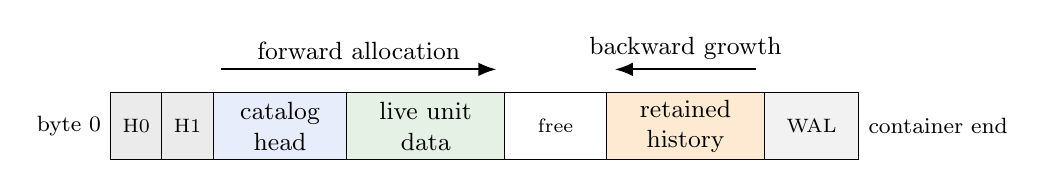
\begin{tikzpicture}[x=1cm,y=0.85cm,font=\small]
    \draw[fill=black!8] (0,0) rectangle (0.65,1);
    \draw[fill=black!8] (0.65,0) rectangle (1.3,1);
    \draw[fill=RoyalBlue!12] (1.3,0) rectangle (3.0,1);
    \draw[fill=ForestGreen!12] (3.0,0) rectangle (5.0,1);
    \draw[fill=white] (5.0,0) rectangle (6.3,1);
    \draw[fill=BurntOrange!15] (6.3,0) rectangle (8.3,1);
    \draw[fill=black!5] (8.3,0) rectangle (9.5,1);

    \node[font=\scriptsize] at (0.325,0.5) {H0};
    \node[font=\scriptsize] at (0.975,0.5) {H1};
    \node[align=center] at (2.15,0.5) {catalog\\head};
    \node[align=center] at (4.0,0.5) {live unit\\data};
    \node[font=\scriptsize] at (5.65,0.5) {free};
    \node[align=center] at (7.3,0.5) {retained\\history};
    \node[font=\scriptsize] at (8.9,0.5) {WAL};

    \draw[->,>=Latex,thick] (1.4,1.35) -- (4.9,1.35)
      node[midway,above] {forward allocation};
    \draw[->,>=Latex,thick] (8.2,1.35) -- (6.4,1.35)
      node[midway,above] {backward growth};
    \node[anchor=east,font=\footnotesize] at (0,0.5) {byte 0};
    \node[anchor=west,font=\footnotesize] at (9.5,0.5) {container end};
  \end{tikzpicture}
  \caption{Schematic v12 physical layout, not to scale.  Two fixed 4-KiB
  header slots alternate as the publication point.  Catalog and live regions
  allocate from the low end, while retained history grows down from the
  high end.  Their gap is available capacity.  When asynchronous writes are
  enabled, a fixed WAL reservation occupies the top of the container and the
  history frontier grows below it.}
  \label{fig:container-layout}
\end{figure}

\Cref{fig:container-layout} makes the independent growth directions and
publication slots explicit.  A collision between the forward and backward
frontiers grows the container rather than allowing the regions to overlap.

Superseded current fragments become self-describing history records when they
must survive.  Retention can thin or explicitly evict unpinned history, and
released ranges can be trimmed.  Limited defragmentation relocates only state
whose history and pin relationships remain valid.  This is not a wandering
log and has no background segment cleaner, but it does have explicit retention,
reclamation, defragmentation, and trim operations.

\subsection{Version-Vector Synchronization and Strains}
\label{subsec:sync}

Synchronization first compares unit version vectors and fragment-dot maps.  For
one fragment position $f$, let $d_L=M_L[f]$ and $d_P=M_P[f]$ be the local and
peer dots.  \sfs{} classifies the position as follows:

\begin{equation}
\operatorname{choose}(f)=
\begin{cases}
L, & d_L=d_P,\\
L, & VV_L\text{ has observed }d_P,\\
P, & VV_P\text{ has observed }d_L,\\
\mathit{conflict}, & \text{otherwise.}
\end{cases}
\end{equation}

The first case is identical state.  In the next two cases, one version vector
witnesses the other dot, so choosing the witnessing side selects a causal
descendant rather than discarding concurrent information.  In the final case
neither side witnesses the other dot.  Selecting either would lose an unseen
update, so the safe result is conflict retention.  Causal dominance and version
vector join are independent of which replica is called local, idempotent, and
commutative.  Replicas presented with the same frontier therefore select the
same non-conflicting fragments and joined vector.

If no position is classified as a conflict, the result selects the indicated
fragments and joins the version vectors.  In particular, two replicas that
modify disjoint fragments from a shared base converge without a
content-specific merge algorithm.  If any position contains mutually unseen
dots, \sfs{} preserves both unit heads as concurrent \emph{strains}.  This is a
same-fragment write conflict, not necessarily a byte collision: two disjoint
byte ranges inside one fragment still produce a strain.  Mounted clients expose
the condition through the \texttt{user.sfs.conflict} extended attribute and the
tooling provides explicit resolution operations.

\Cref{fig:fragment-merge} illustrates the disjoint case and its same-position
boundary.

\begin{figure}[t]
  \centering
  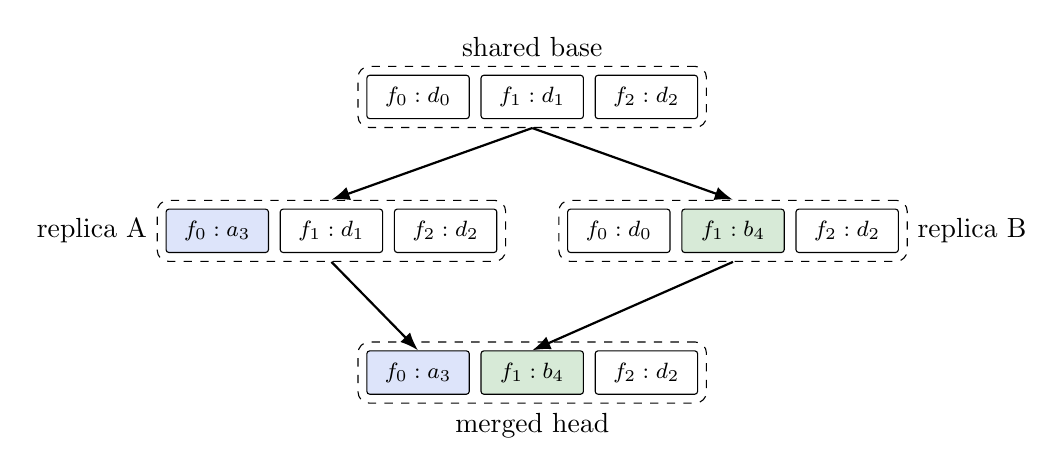
\begin{tikzpicture}[
    frag/.style={draw, rounded corners=1pt, minimum width=1.3cm,
                 minimum height=0.55cm, font=\footnotesize},
    changeda/.style={frag, fill=RoyalBlue!18},
    changedb/.style={frag, fill=ForestGreen!18},
    group/.style={draw, dashed, rounded corners, inner sep=3pt},
    flow/.style={->, >=Latex, thick}]
    \node[frag] (base0) at (0.7,2.6) {$f_0:d_0$};
    \node[frag] (base1) at (2.15,2.6) {$f_1:d_1$};
    \node[frag] (base2) at (3.6,2.6) {$f_2:d_2$};
    \node[group, fit=(base0)(base2), label=above:{shared base}] (base) {};

    \node[changeda] (a0) at (-1.85,0.9) {$f_0:a_3$};
    \node[frag] (a1) at (-0.4,0.9) {$f_1:d_1$};
    \node[frag] (a2) at (1.05,0.9) {$f_2:d_2$};
    \node[group, fit=(a0)(a2), label=left:{replica A}] (agroup) {};

    \node[frag] (b0) at (3.25,0.9) {$f_0:d_0$};
    \node[changedb] (b1) at (4.7,0.9) {$f_1:b_4$};
    \node[frag] (b2) at (6.15,0.9) {$f_2:d_2$};
    \node[group, fit=(b0)(b2), label=right:{replica B}] (bgroup) {};

    \node[changeda] (m0) at (0.7,-0.9) {$f_0:a_3$};
    \node[changedb] (m1) at (2.15,-0.9) {$f_1:b_4$};
    \node[frag] (m2) at (3.6,-0.9) {$f_2:d_2$};
    \node[group, fit=(m0)(m2), label=below:{merged head}] (merged) {};

    \draw[flow] (base.south) -- (agroup.north);
    \draw[flow] (base.south) -- (bgroup.north);
    \draw[flow] (agroup.south) -- (m0.north);
    \draw[flow] (bgroup.south) -- (m1.north);
  \end{tikzpicture}
  \caption{Fragment-causal merge from a shared base.  A replaces position
  \(f_0\) and B independently replaces \(f_1\).  At each changed position the
  writer's new dot causally dominates the other replica's base dot, so the
  merged head contains both updates.  If both replicas instead placed mutually
  unseen dots at the same position, the final case of
  \(\operatorname{choose}\) would retain the two unit heads as strains.}
  \label{fig:fragment-merge}
\end{figure}

We use \emph{strain} for a coexisting head of one logical unit.  Unlike a
repository branch, it does not name a repository-wide line of development.
Unlike a server fork, it does not imply equivocation by the transport.  It is
the retained, user-resolvable consequence of mutually unseen dots at one or
more positions.

Record projections are transferred before or alongside their missing payload
fragments.  A receiving engine may temporarily represent a remote-selected
fragment as a hole and fill it from the transport.  The transport retains a
frontier of pairwise-concurrent record projections rather than a single
last-writer-wins value, so a third replica can discover every unresolved side
from any peer that has observed it.

\subsection{One Protocol for SaaS and Live Peers}
\label{subsec:transport}

All sync intelligence remains in the engine behind a transport interface.  The
interface lists unit frontiers, tests and transfers fragment objects keyed by
$(\mathit{account},\mathit{uuid},f,d_f)$, exchanges encrypted record
projections, and carries capability, writer-set, and key-grant objects.  It does
not expose filesystem operations to the service.

The hosted implementation is a multi-tenant opaque store.  It authenticates
accounts with SRP-6a, derives account scope from the bearer token rather than a
client-supplied path, and persists opaque blocks and record frontiers.  Version
vectors remain visible because the service maintains causal frontiers.  The
service also observes account identifiers, unit UUIDs, fragment indices and
versions, object sizes and counts, timing, and access patterns.  It does not
receive VFS paths, file metadata plaintext, content plaintext, or the client
root key in an encrypted profile.

A live peer implements the same interface directly over an open \sfs{} engine.
Transport calls become manifest projection, fragment export/import, and record
frontier export/import.  No second reconciliation algorithm is introduced.  A
network peer authenticates possession of a root-key-derived P2P key using a
single-use challenge.  Key grants are themselves container units and therefore
propagate through hosted or peer topologies.  The service is thus a replaceable
availability and rendezvous component rather than the authority for filesystem
semantics.

\subsection{Encryption and Multi-Writer Authorization}
\label{subsec:crypto}
\label{subsec:multiwriter}

A password is stretched with Argon2id into a 32-byte root key.  Domain-separated
derivations produce the metadata key, header-MAC key, and one container-level
key for each cryptographic content suite: 32 bytes for GCM and 64 bytes for XTS
(two AES-256 halves).  These keys are suite-specific but not fragment-specific.
Fragment context supplies the nonce or tweak.  Unit records, catalog nodes,
filesystem metadata, paths, writer sets, and key material stored in the
container are AES-GCM protected in v12.  Content is
encoded per fragment as AES-256-GCM, AES-256-XTS, or plaintext.  GCM provides
confidentiality and authentication.  XTS is length-preserving confidentiality
only.  Plaintext is an explicit benchmark/trusted-media mode.  Fragment context
binds UUID, position, causal version, and key epoch into nonce/tweak derivation.

\begin{table}[t]
  \centering
  \small
  \caption{Content-suite claim boundary in v12.  Metadata remains AES-GCM in
  every row.  WriterSet is an additional requirement for the secure hosted
  profile.}
  \label{tab:cipher-profiles}
  \begin{tabular}{@{}llll@{}}
    \toprule
    Content & Confidential & Authenticated & Intended role \\
    \midrule
    GCM & yes & yes & secure hosted/application profile \\
    XTS & yes & no & compatibility and performance mode \\
    \textsc{none} & no & no & trusted-media and benchmark mode \\
    \bottomrule
  \end{tabular}
\end{table}

The paper's end-to-end-encrypted deployment profile means GCM content plus
WriterSet signing.  In that profile neither the hosted service nor its at-rest
database receives the client root key or decryptable VFS state.  TLS protects
the wire hop, but confidentiality from the service follows from the client-side
container encryption, not from TLS.  This is client-side-encrypted storage
rather than cryptographic zero knowledge because the synchronization metadata
listed above remains visible.

WriterSet containers have an Ed25519 owner key and an owner-signed, monotone
writer-set object.  Members sign the replica-invariant logical portion of a unit
record: UUID, fragment dots, version vectors, geometry, and an optional
application head.  Replica-local locations, parent pointers, pins, cipher
encodings, and strain addresses are excluded so relocation, re-ciphering, and
cross-replica import do not invalidate signatures.  The signature consequently
authorizes and attributes a logical record frontier.  It is not a per-fragment
provenance proof or a content digest.  GCM authenticates content in the secure
profile.

Removal is represented by a tombstone and is coupled to a higher key epoch.
Root-key rotation re-encrypts live content, metadata, catalogs, and unresolved
strains before atomically publishing the new epoch.  New root keys are sealed
to retained members with ephemeral X25519/HKDF/AES-GCM grants.  A peer that has
not yet received its matching grant remains safely on its old epoch.  A retained
peer can adopt the new key and writer set in one local publication.  Rotation is
forward-only in v12: pre-rotation parent history and retention pins are not
carried across the key boundary, while live conflict strains are.


\section{Implementation}
\label{sec:impl}

The RC1 artifact is a Rust workspace plus an independent Linux kernel
implementation. Tagged source and release artifacts are available from the
project repository.  Published Cargo packages use the \texttt{zero-sfs-*}
prefix~\citep{SfsArtifact2026}. \Cref{tab:artifact} summarizes the paths
relevant to this paper. Operational service features such as proxy deployment,
rate limiting, health endpoints, and recovery-code handling are implemented
but are not treated as research contributions.

\begin{table}[t]
  \centering
  \small
  \caption{Principal implementations over the v12 logical format.}
  \label{tab:artifact}
  \begin{tabular}{@{}lll@{}}
    \toprule
    Component & Physical backend & Role \\
    \midrule
    Rust core & file or memory & format, MVCC, crypto, recovery \\
    Linux kernel VFS & raw block device & native mounted filesystem \\
    FUSE adapter & container file on host FS & portable mounted filesystem \\
    Sync/SaaS & opaque network objects & hosted or peer replication \\
    WebAssembly adapter & in-memory image & browser/application VFS API \\
    C ABI/tools & Rust core & embedding, inspection, repair \\
    \bottomrule
  \end{tabular}
\end{table}

\subsection{Rust Format Authority}

The core engine forbids unsafe Rust and does not depend on a general-purpose
serialization framework.  Header, catalog, unit-record, writer-set, key-grant,
WAL, and eviction formats are length-checked binary codecs.  The file backend
uses positioned reads and writes.  The memory backend exposes the same byte
image through an in-memory vector.  Both follow the same open path, including
header authentication, catalog and allocator reconstruction, and WAL recovery.

The current reader accepts exactly format v12.  This clean-cut policy prevents
silent interpretation of development-era formats, but it is not a format
stability promise: no migration implementation is included.  Cross-language
constants and derivations, including the fragment-size staircase and cipher
contexts, are recorded as golden vectors.  The artifact also includes hostile
decoder tests and six coverage-guided fuzz targets for unit records, commits,
eviction records, writer sets, key grants, and NoSQL records.

\subsection{Raw-Device Linux VFS}

The kernel path is an independent C implementation mounted directly on a block
device.  It parses and publishes the same headers, catalogs, unit records,
fragment geometry, encryption contexts, and writer state as the Rust engine.
The driver integrates with the Linux page cache and provides the broad VFS
subset needed by the evaluated filesystem: files and directories, read/write,
truncate, rename, symlinks, attributes, extended attributes and ACLs, and
filesystem statistics.  The implementation is intentionally described as an
experimental VFS rather than as complete POSIX conformance.  Remaining alias and
link-count semantics are listed in \cref{sec:discussion}.

Keeping the driver independent is useful evidence for format specificity: the
kernel does not call into the Rust engine or mount a userspace proxy.  C/Rust
round-trip fixtures and byte-level known-answer vectors guard the shared
format.  Loaded-module, target-kernel, and KASAN campaigns remain external
artifact gates because hosted CI can compile but cannot safely load the module
or provide a disposable block device.

\subsection{Portable Host-File VFS}

The FUSE adapter embeds the Rust engine and stores one container file on a host
filesystem.  This adds a userspace transition and a second filesystem layer,
but works without a kernel module and carries the complete engine feature set.
The adapter coalesces writes into explicit publication batches and implements
sequence-detecting read-ahead: a handle prefetches only after observing
sequential access, avoiding the prior random-read overfetch and memory pressure.
The same adapter layer contains macFUSE and WinFsp integration points, although
this paper evaluates only the Linux FUSE path and does not claim real-platform
validation for macOS or Windows.

The mounted surface exposes conflicts through extended attributes and maps
engine integrity failures to I/O errors rather than returning fabricated data.
FUSE and the kernel driver must not mount the same image concurrently: the
userspace advisory lock is taken on the container-file inode and cannot
coordinate with a block-device mount.

\subsection{Encrypted Hosted Storage and Peer Service}

The synchronization crate contains the transport-independent reconciliation
engine.  Its in-memory transport is used for model and integration tests.  The
production network client uses a compact binary wire format over TLS.  Batched
fragment requests amortize HTTP and authentication overhead.  The hosted
service supports direct TLS over HTTP/1.1, HTTP/2, and HTTP/3, or operation
behind a trusted TLS-terminating proxy.  Authentication uses SRP-6a followed by
scoped bearer tokens.  No password-equivalent value is sent during login.

Persistent server state is itself stored through an \sfs{} engine for account
and frontier metadata, with a separate append-oriented block-blob store for
large opaque payloads.  This is server-side operational encryption in addition
to, not a replacement for, the client's end-to-end container encryption.  The
service can verify signed record projections when writer enforcement is
enabled.  The deployed binary enables that policy by default.  It still cannot
interpret client paths, VFS metadata, or content in the secure profile.

The peer daemon reuses the hosted \texttt{/v1} wire and network client but
replaces the server store with an \texttt{EngineTransport} over a live
container.  A root-key-possession challenge replaces SRP.  This implementation
choice is what makes hosted and peer synchronization two topologies of one
protocol rather than two replication systems.

\subsection{WebAssembly and Embedded VFS}

The WebAssembly crate exposes container creation, password and raw-key opening,
file and directory creation, offset writes, truncate, read, list, and snapshot
operations through \texttt{wasm-bindgen}.  It uses the core memory backend, so
the byte vector returned by \texttt{snapshot} is the same container image that
the file backend and native VFS implementations open.  Password salts and
nonces route through the browser randomness backend.  The core disables its
native thread-based decrypt pool for wasm and uses the serial path.

The implementation establishes a source-level browser boundary, not yet a
browser deployment result.  Native tests exercise the wasm-selected core logic,
but the RC1 evidence does not include a hosted \texttt{wasm32-unknown-unknown}
build, JavaScript end-to-end test, or persistent OPFS/IndexedDB backend.  We
therefore call the bindings experimental throughout the paper.  Their relevance
is architectural: an application can own a complete encrypted VFS image and
hand only encrypted synchronization objects to the service, using the same
format and key model as the native clients.

\subsection{Artifact Evidence}

The source tree contains unit, property, integration, network, crash-seam, and
cross-format tests.  Relevant fixtures cover crashes before header publication
and round trips for GCM, XTS, and plaintext.  Further scenarios exercise signed
record and writer-set rejection, concurrent frontiers, third-replica
convergence, hosted and peer transports, and C/Rust golden vectors.  These tests
are evidence for implemented paths, not a formal proof of correctness or an
independent security audit.


\section{Evaluation}
\label{sec:eval}

The evaluation asks four deliberately bounded questions.  \textbf{RQ1:} Do
independent replicas exhibit the advertised disjoint-fragment merge,
same-fragment strain, resolution, and transport behavior in controlled
end-to-end scenarios?  \textbf{RQ2:} Does the native kernel path remain
competitive with the conventional Linux block stack for sequential I/O?
\textbf{RQ3:} What portability cost does the FUSE path impose relative to a
FUSE filesystem with comparable encryption?  And \textbf{RQ4:} are the
reported throughput samples free of the process leaks, out-of-memory
terminations, and silent zero results that can invalidate a long storage
campaign?  We do not use these experiments to answer metadata-workload,
multi-client scalability, or non-loopback LAN/WAN synchronization questions.

\subsection{Functional Multi-Replica Evidence}
\label{subsec:eval-mechanisms}

The RC1 test matrix includes deterministic end-to-end scenarios for the
distributed mechanisms, summarized in \cref{tab:mechanism-evidence}.  Each has
a binary acceptance oracle over exact bytes, frontier cardinality, or an
expected authorization result; none derives latency, throughput, conflict
probability, or scale from the scenario.

\begin{table}[t]
  \centering
  \small
  \setlength{\tabcolsep}{4pt}
  \caption{Controlled mechanism scenarios in the RC1 artifact.  These are
  correctness fixtures, not workload or scalability measurements.}
  \label{tab:mechanism-evidence}
  \begin{tabular}{@{}p{0.19\linewidth}p{0.22\linewidth}p{0.50\linewidth}@{}}
    \toprule
    Mechanism & Controlled topology & Acceptance oracle \\
    \midrule
    Disjoint writes &
      two replicas, opaque local transport &
      both replicas read the exact combined fragments, expose no conflict, and
      remain stable on a second sync \\
    Same-fragment writes &
      two clients, hosted TLS service &
      both retain two byte-exact strains; a selected resolution propagates and
      collapses the remote frontier to one \\
    Late observer &
      two writers plus a fresh third client, hosted TLS service &
      the third client reconstructs exact units and both unresolved strains;
      a later fresh client observes the resolved frontier \\
    Live-peer topology &
      two containers, TLS on ephemeral loopback &
      one sync transfers each peer's distinct unit in both directions;
      wrong-key and unauthenticated access are rejected \\
    Hosted authorization &
      WriterSet clients and enforcing service &
      member frontiers are accepted; non-member and revoked-writer frontiers
      are rejected; stored-byte scans contain no injected plaintext markers \\
    \bottomrule
  \end{tabular}
\end{table}

The fixtures are implemented under \path{crates/sfs-sync/tests} and
\path{crates/sfs-saas/tests} as
\texttt{conflict\_e2e}, \texttt{net\_e2e},
\texttt{p2p\_net\_e2e}, \texttt{enforcement\_e2e}, and
\texttt{zk\_proof\_e2e}.  Together they answer RQ1 at the mechanism level:
the advertised reconciliation outcomes cross both an opaque hosted transport
and a live network peer, and an unresolved frontier remains discoverable by a
client that did not participate in the conflict.  They do not answer how often
those outcomes occur in a repository or how their cost grows with agents,
files, latency, or history.

The artifact also guards the re-chunk boundary called out by the geometry
design.  Functional fixtures grow a unit from 4-KiB to 256-KiB fragments,
require byte-exact content, fresh causal dots, preserved pinned history,
publication-safe failure, and successful reopen.  A separate physical-footprint
regression appends 512-KiB chunks to 32 MiB.  The fixture records a before/after
observation of 62 MiB of allocated blocks, or \(1.94\times\) logical size,
versus 146 MiB (\(4.58\times\)) for the superseded implementation that retained every
re-chunked generation; the guard requires less than \(2.5\times\).  This
\texttt{st\_blocks} high-water proxy includes freed but not hole-punched
intermediate generations.  It is neither a transition-latency result nor a
long-term aging experiment, and the paper does not treat it as part of the
fault-gated throughput campaign below.

\subsection{Method}
\label{subsec:eval-method}

We compare within execution surfaces, not across them.  The kernel module uses
a raw block device and is compared with ext4 on that device for plaintext and
ext4 over LUKS for encrypted I/O.  The FUSE daemon stores an \sfs{} container
on ext4 and is compared with fuse2fs for plaintext and gocryptfs for encrypted
I/O.  Thus each ratio has a baseline in the same kernel/userspace class; a
kernel-to-FUSE ratio would answer a different question.

The published campaign used kernel artifact \texttt{4cb3e28} and FUSE artifact
\texttt{4a41dbeb}.  It ran on a Linux benchmark VM backed by a Samsung 960 EVO,
using \texttt{fio}'s single-threaded \texttt{psync} engine.  Each cell is the
arithmetic mean of ten fault-free runs.  The 14 request sizes range from 4 KiB
through 2047 MiB; files are 1 GiB except for the 2047-MiB request, which uses a
2-GiB file.  The 2047-MiB endpoint stays below Linux's
\texttt{MAX\_RW\_COUNT}; literal 2- and 4-GiB single requests fail for ext4 as
well and are therefore not \sfs{} limits.

Every run starts with block discard, cache dropping, and a fresh mount.  Read
results are consequently cold-cache results.  The fixture inspects kernel
messages, OOM events, leaked daemons, and available memory after each run and
excludes a run on any such fault.  The final campaign reported zero faults, so
all ten samples entered every cell.  Source, on-filesystem, and cold-read hashes
were also compared for the plaintext, XTS, and GCM paths before accepting the
campaign.

The checked-in aggregate is
\texttt{docs/perf/perf-report-2026-07-20.html}.  For compact comparison,
Tables~\ref{tab:kernel-perf} and
\ref{tab:fuse-perf} report the geometric mean of the 14 per-size ratios
\[
  R_{\mathrm{geo}} =
  \exp\!\left(\frac{1}{14}\sum_{i=1}^{14}
  \ln\frac{\overline{x}_{\sfs{},i}}{\overline{x}_{\mathrm{base},i}}\right),
\]
where each \(\overline{x}\) is the arithmetic mean for one cell.  This gives
equal multiplicative weight to each request size.  The repository report
contains every per-size cell, but currently archives aggregates rather than
the ten raw samples and their health logs; this prevents confidence intervals
or an independent reanalysis of run-level variance.

\subsection{Kernel Path}
\label{subsec:eval-kernel}

\begin{table}[t]
  \centering
  \caption{Kernel-path throughput relative to its group baseline.  Values are
  geometric means over 14 request sizes; larger is better.}
  \label{tab:kernel-perf}
  \begin{tabular}{lllr}
    \toprule
    Content & Operation & Baseline & \sfs{}/baseline \\
    \midrule
    Plain & write & ext4-raw & \(1.22\times\) \\
    Plain & cold read & ext4-raw & \(0.98\times\) \\
    XTS & write & LUKS-ext4 & \(0.99\times\) \\
    GCM & write & LUKS-ext4 & \(0.98\times\) \\
    XTS & cold read & LUKS-ext4 & \(1.20\times\) \\
    GCM & cold read & LUKS-ext4 & \(1.11\times\) \\
    \bottomrule
  \end{tabular}
\end{table}

Table~\ref{tab:kernel-perf} answers RQ2 for this sequential, queue-depth-one
workload.  Plain writes are faster than ext4 on average, while plain reads and
encrypted writes are at parity under a \(0.98\times\) convention.  Encrypted
cold reads exceed the LUKS-ext4 baseline for both ciphers.  These are
geometric summaries, not universal dominance: individual cells can lose.  In
particular, the 2047-MiB encrypted-write endpoint is approximately
\(0.81\times\) LUKS.  The result supports the narrower claim that native
fragment versioning and authenticated metadata do not introduce an inherent
sequential-throughput penalty on this device and workload.

\subsection{FUSE Path}
\label{subsec:eval-fuse}

\begin{table}[t]
  \centering
  \caption{FUSE-path throughput relative to its group baseline, computed as in
  Table~\ref{tab:kernel-perf}.}
  \label{tab:fuse-perf}
  \begin{tabular}{lllr}
    \toprule
    Content & Operation & Baseline & \sfs{}/baseline \\
    \midrule
    Plain & write & fuse2fs & \(3.11\times\) \\
    Plain & cold read & fuse2fs & \(1.70\times\) \\
    XTS & write & gocryptfs & \(0.87\times\) \\
    GCM & write & gocryptfs & \(0.85\times\) \\
    XTS & cold read & gocryptfs & \(0.38\times\) \\
    GCM & cold read & gocryptfs & \(0.33\times\) \\
    \bottomrule
  \end{tabular}
\end{table}

The portable path has two distinct regimes.  Sequence-detecting read-ahead
lets plaintext \sfs{} outperform fuse2fs for both reads and writes, showing
that the FUSE boundary alone is not the limiting factor.  Encrypted writes are
13--15\% below gocryptfs.  Encrypted cold reads are the clear remaining
weakness: XTS reaches \(0.38\times\) and GCM \(0.33\times\) of gocryptfs in the
geometric mean.  At large requests the corresponding ratios rise only to
approximately \(0.43\times\) and \(0.38\times\).

Profiling attributes approximately 40\% of the encrypted-read time to
parallel AES-NI decryption, 19\% to container reads, and 32\% to FUSE reply,
system-call, and backpressure work, with the remainder in buffer movement.
This is a mixed end-to-end userspace ceiling, not evidence for one removable
\texttt{splice} or library bottleneck: the plaintext path reaches roughly
1.5 GB/s through the same reply implementation, and the compared gocryptfs
read path does not establish a zero-copy explanation.  Closing the gap would
therefore require a separate buffer-ownership and pipeline study.  The result
answers RQ3 honestly: FUSE is a useful portable path, but it is not the
performance path for encrypted sequential reads in this release.

\subsection{Fault Discipline and Scope}
\label{subsec:eval-validity}

A preliminary campaign was discarded in full after externally unmounted FUSE
daemons failed to exit, accumulated, and eventually caused OOM kills and
zero-valued cells.  No number from that campaign appears here.  The daemon exit
was corrected and the per-run health gate described above was added before the
reported campaign.  This experience is why RQ4 is part of the evaluation: ten
repetitions do not improve a result if failed runs silently enter the mean.

The remaining validity limits are material.  The campaign uses one VM, one
SSD, buffered single-threaded sequential I/O, and throughput rather than tail
latency.  It does not exercise random I/O, metadata-heavy application traces,
multiple queue depths, many writers, network delay, link rate,
synchronization volume, or conflict frequency.  The data therefore validate a
local data path and expose one FUSE weakness; they do not by themselves
validate the broader agentic-time workload at scale.


\section{Related Work}
\label{sec:related}

% The subsections position the shared fragment representation against its
% neighboring research lines. They are not a capability-scorecard.

% ── Versioning filesystems ─────────────────────────────────────────────────
\subsection{Versioning Filesystems}
\label{subsec:rw-versioning}

Prior versioning filesystems fall into three broad families. \emph{Per-write /
comprehensive} systems
keep a version on every write: Elephant retains all versions and lets
user policy decide what to forget~\citep{Santry1999Elephant}. CVFS versions at
write granularity with space-efficient multiversion metadata for a fixed
security window~\citep{Soules2003CVFS}. Wayback and VersionFS realize the same
idea as a user-level undo log and a stackable
layer~\citep{Cornell2004Wayback, MuniswamyReddy2004VersionFS}. \emph{Snapshot /
copy-on-write} systems version at point-in-time, filesystem-wide granularity:
WAFL duplicates the root inode~\citep{Hitz1994WAFL}, ZFS and Btrfs snapshot
whole datasets/subvolumes over CoW trees~\citep{Rodeh2013Btrfs}, and ext3cow
adds epoch snapshots to ext3~\citep{Peterson2005Ext3cow}. \emph{Content-addressed
/ git-like} systems version through immutable objects and discrete commits: Ori
gives a filesystem a git-style replicated, integrity-checked
history~\citep{Mashtizadeh2013Ori}, and ForkBase pulls git-conformant branching
into a storage substrate~\citep{Lin2020ForkBase}.

\sfs{} differs from all three, but does not claim to be the first filesystem
with native multiversion structures. In particular, CVFS uses journal-based
multiversion B-trees for filesystem metadata~\citep{Soules2003CVFS}. In \sfs{},
versioning is neither an overlay
(Wayback/VersionFS), a filesystem-wide snapshot (WAFL/ZFS/Btrfs/ext3cow), nor a
separate object store (Ori/ForkBase/git): each unit carries its own
continuously advanced fragment lineage as the \emph{native} on-disk model, with
named commits as retention-protected fixpoints layered over the running history
(\cref{subsec:mvcc}). Multiversion concurrency control is well established in
databases. Recent work extends it to disaggregated
memory~\citep{Zhang2024Motor}. The narrower gap \sfs{} targets is a per-file
fragment version map that is simultaneously the unit of history,
synchronization, and sub-file conflict handling, combined with the encrypted
multi-writer and cross-surface container design.

% ── CoW, crash consistency, allocator ──────────────────────────────────────
\subsection{Copy-on-Write, Crash Consistency, and Allocation}
\label{subsec:rw-cow}

Crash-consistency mechanisms split into journaling, explicit dependency
ordering, and atomic root publication.  Journaling ranges from
ext3/4 to optimizations that decouple ordering from durability
(OptFS~\citep{Chidambaram2013OptFS}). Ordering approaches include soft
updates~\citep{Ganger2000SoftUpdates}, Featherstitch's generalized
dependencies~\citep{Frost2007Featherstitch}, and, recently, SquirrelFS, which
encodes update ordering in Rust's typestate and checks it at compile
time~\citep{LeBlanc2024SquirrelFS}. They avoid a journal but have no single atomic
point. \sfs{} uses the third mechanism for publication: the committed root is a
sequence-wins choice between two alternating header slots. This is not a
journal-free-system claim: an optional WAL serves asynchronous writes, and
in-place overwrite recovery uses undo records in the eviction tail. WAFL's two
alternating \texttt{fsinfo} blocks~\citep{Hitz1994WAFL} are the closest
precursor to the root publication. ZFS's uberblock ring uses the same principle.
Our novelty is not that commit pattern but its combination with
\emph{fragment-granular} CoW over a flat three-region allocator: WAFL, ZFS, and
Btrfs shadow tree paths recursively up to the root,
which measurably amplifies writes~\citep{Rodeh2013Btrfs}. \sfs{} does not place
file content in such a filesystem-wide CoW tree, although its key and identity
catalog tries still incur their own CoW update cost
(\cref{subsec:commit,subsec:alloc}). On space management, LFS and
its flash/NVM successors (F2FS~\citep{Lee2015F2FS}, NOVA~\citep{Xu2016NOVA}) are
log-structured with a cleaner/GC.  \sfs{} has no background wandering cleaner:
fixed regions (catalog head, live units, eviction tail) replace the wandering
log, while retention expiry, reclamation, defragmentation, and trim are explicit
operations.  The eviction-tail region has no direct analogue in that
literature. WineFS's finding that alignment and aging affect fragmentation
substantially~\citep{Kadekodi2021WineFS} reinforces the need to evaluate the
long-term behavior of this simpler allocator separately.

% ── Chunking ────────────────────────────────────────────────────────────────
\subsection{Chunking: Content-Defined versus Fixed-Size}
\label{subsec:rw-chunking}

Content-defined chunking (CDC), introduced by LBFS~\citep{Muthitacharoen2001LBFS}
and since accelerated by Data Domain~\citep{Zhu2008DataDomain} and the FastCDC
line~\citep{Xia2016FastCDC}, sets chunk boundaries by a rolling hash so that an
inserted byte does not shift all following boundaries. The trade-off is
content-dependent boundaries and a rolling-hash scan. CDC is deterministic for
a fixed input and algorithm. Its boundaries are content-dependent, not random.
\sfs{} deliberately rejects CDC in favor of fixed-size fragments with a
$\sqrt{\cdot}$-shaped schedule: within a size band, fixed boundaries give a
constant-time position$\rightarrow$fragment mapping (fragment $n$ of a version
maps to fragment $n$ of the next), with no rolling-hash scan. A sync round still
scans the unit manifests and fragment-version vectors, so its metadata work is
linear in the number of units and fragments. Normal steady-state sync transfers
changed or missing fragments. At a fragment-size band transition, \sfs{}
re-chunks the unit.
Advances in CDC \emph{throughput} do not change this content-dependence trade-off.
The Merkle-/content-addressed tradition (Venti~\citep{Quinlan2002Venti},
git, IPFS~\citep{Benet2014IPFS}, Tahoe-LAFS~\citep{WilcoxOHearn2008Tahoe}) informs
\sfs{}'s Merkle-like catalog trie, but \sfs{} keeps identity+version addressing
for data blocks rather than pure content addressing, precisely because it
synchronizes mutable versions rather than stacking immutable snapshots.

% ── Replication and conflict resolution ────────────────────────────────────
\subsection{Optimistic Replication and Conflict Resolution}
\label{subsec:rw-replication}

\sfs{}'s synchronization descends from version vectors~\citep{Parker1983VersionVectors}
and the optimistic-replication filesystems built on them: Coda's disconnected
operation~\citep{Kistler1992Coda}, Ficus's peer replication with VV conflict
detection~\citep{Reiher1994Ficus}, Bayou's application-defined merge
procedures~\citep{Terry1995Bayou}, and Ivy's per-participant logs in a
DHT~\citep{Muthitacharoen2002Ivy}. Across this family, \emph{content} conflicts
within a file are left whole-file and usually manual (Ficus auto-merges only
directory structure, and Ivy needs a conflict tool). At the other pole, CRDTs
eliminate conflicts algebraically~\citep{Shapiro2011CRDT}: JSON-CRDT/Automerge
converge nested documents~\citep{Kleppmann2017JSONCRDT}, ElmerFS models
filesystem structures as CRDTs over a CRDT
store~\citep{Elmerfs2021}, at the price of per-element metadata,
tombstones, and sometimes counter-intuitive auto-resolutions. \sfs{} sits
between the two: version-vector sync with \emph{block-granular} auto-merge.
With strain splits, concurrent edits to different fragments of the same file
merge automatically, while concurrent updates to the same fragment remain a
conflict even when the changed byte ranges inside it do not overlap.  The
conflict is surfaced as a \texttt{user.sfs.conflict} xattr. This fills the gap
the VV filesystems leave (sub-file content merge) without adopting CRDT
machinery.

% ── Portable encrypted VFS and cloud substrates ────────────────────────────
\subsection{Portable Encrypted VFS and Cloud Substrates}
\label{subsec:rw-vfs}

WNFS is the closest architectural neighbor on the web-facing side: it is a
versioned, content-addressed, encrypted filesystem designed for offline
collaboration, untrusted storage, and WebAssembly, and models the tree as a
state-based CRDT~\citep{WNFSspec}.  Peergos likewise combines client-side
encryption, protected metadata, capability sharing, cloud or peer storage, and
web and desktop clients~\citep{Peergos}.  These systems demonstrate that an
encrypted application-owned filesystem is a useful web abstraction.  \sfs{}
does not claim that category.  Its narrower distinction is to carry one
position-addressed fragment/version representation through ordinary file APIs,
a raw-device kernel implementation, FUSE, an application VFS, and an
experimental wasm binding.  It preserves concurrent same-fragment branches
rather than making the entire tree a CRDT.

At the infrastructure scale, OceanStore treats persistent encrypted objects as
the basis for global storage~\citep{Kubiatowicz2000OceanStore}, while Ceph
builds file, block, and object services above a distributed object
store~\citep{Weil2006Ceph}.  \sfs{} borrows the unifying-substrate ambition but
not their scale claim: its hosted service is an untrusted relay for the same
client-owned records used locally, and the present evaluation contains neither
a storage cluster nor a multi-client scalability experiment.  The result is a
backend-neutral VFS boundary, not a replacement for a distributed object-store
control plane.

% ── Cryptographic / untrusted storage ──────────────────────────────────────
\subsection{Cryptographic and Untrusted Storage}
\label{subsec:rw-crypto}

Cryptographic filesystems progress by threat model. Farsite is an important
early combination: it encrypts file data placed on incompletely trusted desktop
machines and uses Byzantine fault tolerance for distributed filesystem
metadata~\citep{Adya2002Farsite}. Local, honest-but-curious
(HbC) systems such as CFS~\citep{Blaze1993CFS}, \texttt{gocryptfs}/eCryptfs,
and dm-crypt/LUKS give at-rest confidentiality for one user, without multi-writer
or sync. Secure-sharing-on-untrusted-storage systems add key management and
revocation: Plutus with lazy revocation via key
rotation~\citep{Kallahalla2003Plutus}, SiRiUS with signed per-file metadata over
an untrusted underlay~\citep{Goh2003SiRiUS}, Cryptree with hierarchical key
derivation~\citep{Grolimund2006Cryptree}, and Key Regression formalizing the
rotation~\citep{Fu2006KeyRegression}. A stronger model assumes an actively
byzantine server and provides \emph{fork consistency}: SUNDR~\citep{Li2004SUNDR}
makes any server equivocation detectable, and SPORC extends this to collaborative
multi-writer apps~\citep{Feldman2010SPORC}. Depot tolerates faulty nodes and
heals forks~\citep{Mahajan2011Depot}. Recent metadata-hiding systems push
further with ORAM (Metal~\citep{Chen2020Metal}, Titanium~\citep{Chen2022Titanium})
or anonymity (Ghostor~\citep{Hu2020Ghostor}), and KBFS signs a recursive root
block for integrity under total server compromise. Cryptanalysis of deployed
end-to-end-encrypted storage~\citep{Backendal2023MEGA, Backendal2024BrokenEcosystem}
motivates the whole line: real providers turn malicious, and the server must
never see keys or paths.

\sfs{} takes the \emph{honest-but-curious} position deliberately, not the
fork-consistency one.  In its secure hosted profile, metadata and content are
client-side AES-GCM encrypted and accepted record frontiers are authorized by
Ed25519 signatures under an owner-signed, epoch-versioned writer set.  The
server receives neither keys, paths, metadata plaintext, nor content plaintext.
This statement does not extend to the selectable XTS or plaintext content
modes: XTS provides confidentiality without authentication, and \textsc{none}
provides neither.  We use \emph{client-side-encrypted storage} rather than the
cryptographic term zero knowledge because the service still observes accounts,
object identifiers, version vectors, counts and sizes, timing, and access
patterns.  The signatures cover logical record frontiers, not a complete
per-fragment provenance proof.

Multi-writer authorization comes from the signed writer set (tombstone
revocation and root-key rotation) rather than from a
fork-consistency protocol or CRDT/OT. Relative to Plutus, revocation is bound to
epochs and the writer set rather than to per-file-group key chains. Relative to
SUNDR/SPORC, \sfs{} does not guarantee detection of a server that withholds or
forks versions. This is an explicit model weakening we defend in \cref{sec:discussion}.
KBFS is a close deployed neighbor~\citep{KeybaseKBFS}. \sfs{} differs in
binding identity to SRP-6a password authentication and a self-contained
container rather than to social sigchains, and in targeting one self-contained
format across kernel, FUSE, and experimental wasm bindings.

Finally, the earlier Self-Certifying File System also used the acronym
SFS~\citep{Fu2000SFS}.  It secured remote access through self-certifying
pathnames and is otherwise unrelated to the artifact described here.  This
paper consistently typesets the present system as \sfs{}.


\section{Discussion and Limitations}
\label{sec:discussion}

\subsection{What the Agentic-Time Claim Means}

The central claim is architectural: causal history, synchronization, and
conflict isolation can share one filesystem representation, so independent
agents need not coordinate every update through an explicit repository commit.
The artifact implements concurrent frontiers, disjoint-fragment merge, retained
strains, and hosted and peer transports.  The controlled multi-replica
scenarios in \cref{subsec:eval-mechanisms} exercise those mechanisms, including
third-replica discovery and resolution propagation, but do not establish how a
real fleet of agents behaves.  The evaluation contains no repository trace,
non-loopback LAN or WAN deployment, conflict-frequency study, or scaling curve
over agents, replicas, files, and retained versions.  We therefore claim a substrate for that
workload, not measured superiority to Git, worktrees, or existing synchronizers
for an end-to-end development task.  Such a study is the most important
remaining evaluation rather than a missing storage feature in RC1.

For the intended workload, the first missing network experiment is a LAN
experiment rather than necessarily a long-haul WAN experiment: colocated
agents and developer machines make 1- and 10-Gbit/s Ethernet the primary
operating range.  Remote and cloud-agent cases add links from roughly
10-Mbit/s constrained upstreams through 10-Gbit/s data-center connectivity.
A useful evaluation should sweep link rate, RTT, and loss independently while
varying writers and changed fragments, then report synchronization completion
time, transferred bytes, CPU cost, and conflict visibility latency.  These are
future evaluation parameters; the loopback TLS scenarios in this paper make no
claim about any point in that matrix.

\subsection{Security Boundary}

The strongest deployment claim is intentionally conditional.  End-to-end
confidentiality and authenticated content require GCM content, the always-GCM
metadata path, and WriterSet enforcement.  XTS content is confidential but
malleable; plaintext content has no cryptographic protection.  Neither mode may
inherit the full secure-SaaS claim merely because it uses the same transport.
Even in the secure profile, the service learns the account, UUIDs, fragment
indices and causal versions, version vectors, sizes, timing, and access
patterns.  \sfs{} is consequently client-side encrypted, not metadata-oblivious
or zero knowledge.

The hosted service is assumed honest-but-curious.  It may reject an
unauthorized record frontier, and GCM rejects modified ciphertext, but no
protocol in v12 detects a service that withholds a recent frontier, presents an
old but valid view, or forks two clients.  The signed writer set provides
authorization, not SUNDR-style fork consistency.  A transparency log,
client-to-client witness exchange, or signed monotone root chain could strengthen
that model, at additional state and availability cost.  Endpoint compromise,
root-key theft, traffic analysis, and denial of service are also outside the
current protection boundary.  No independent cryptographic audit has been
performed.

Key rotation is a forward boundary, not retroactive erasure.  A removed writer
may retain ciphertext and keys obtained before removal.  The live state and
unresolved strains are re-encrypted into the new epoch, but pre-rotation parent
history and pins are not carried across it.  Applications that require one
continuous, decryptable history across revocation need a different archival-key
policy.

\subsection{Granularity, Retention, and Durability}

Fixed positions make offset lookup constant time and let disjoint fragments
merge without a content-specific data type.  They deliberately give up the
insertion stability and cross-file deduplication of content-defined chunking.
Two concurrent edits to different bytes in one fragment still conflict, and a
size-band transition rewrites the complete logical unit under fresh dots and
loses delta reuse against its old geometry.  The artifact's 32-MiB append
regression records the bounded forward-growth case in
\cref{subsec:eval-mechanisms}; it does not measure latency or repeated growth,
shrink, or oscillation around a boundary.  Manifest construction and comparison
are linear in total unit and fragment metadata; only position lookup is
\(O(1)\).  Workloads dominated by insertion shifts or cross-file duplicates
may prefer content-defined chunks or an application CRDT.

History is bounded by policy and key epoch.  Named cuts pin required fragments
against ordinary retention, but they are not an eternal-retention promise.
Reclamation, retention expiry, defragmentation, and trim are explicit; the
artifact has no background cleaner whose aged steady state is evaluated here.
The three-region layout therefore needs long-duration fragmentation and
space-amplification measurements under repeated overwrite, snapshot, sync, and
rotation workloads.

The alternating authenticated header is an atomic publication point, not a
claim that every path is log-free or formally crash-safe.  The asynchronous
mount path uses a WAL and bounded in-place changes use undo records.  The
artifact contains crash-seam tests, but this paper reports no real power-cut or
systematic block-reordering campaign.  Offline scanning is a recovery aid; its
highest-address choice among unrelated orphan records is explicitly heuristic.

\subsection{Surfaces and Format Maturity}

The raw-device driver and FUSE adapter expose a broad useful VFS subset rather
than proven POSIX conformance.  Alias and hard-link accounting remain
incomplete, and the FUSE view reports simplified link counts.  A FUSE mount and
kernel mount must not open the same image concurrently because their lock
domains do not meet.  The Linux kernel path is the evaluated high-performance
encrypted path.  The FUSE encrypted-read deficit in
\cref{subsec:eval-fuse} is characterized but unresolved; it matters when the
portable mount is expected to carry high-throughput encrypted reads.
The profile decomposes \sfs{} itself but does not comparatively instrument
gocryptfs, so it cannot attribute the threefold gap to splice, copying, or one
particular scheduling decision.  Those remain hypotheses for a dedicated
buffer-ownership and pipeline experiment, not findings of this paper.

The wasm adapter currently demonstrates that the core engine can operate on an
in-memory image through a browser-shaped API.  RC1 does not include the
browser-target build and JavaScript end-to-end evidence or a persistent
OPFS/IndexedDB backend needed to call it a deployed web filesystem.  Likewise,
macFUSE and WinFsp integration points are not substitutes for measurements on
macOS and Windows.  These are important execution surfaces, but the paper keeps
them experimental.

Finally, the reader accepts exactly v12 and provides no migration path from
development formats.  A release can reasonably make this clean cut, but a
long-lived application VFS needs a documented compatibility policy, migrations,
and rollback tooling.  The published performance report preserves aggregate
cells but not raw samples and per-run health logs; a durable research artifact
should archive both and bind them to full source and environment manifests.


\section{Conclusion}
\label{sec:conclusion}

\sfs{} began with an agentic-time problem: one evolving project should be
available to many autonomous writers across machines without reducing live work
to manual clones, explicit commits, or last-writer-wins synchronization.  Its
answer is to make a position-addressed fragment map causal.  The same map
materializes current bytes, identifies retained history, names synchronization
payloads, and separates disjoint concurrent changes from same-fragment strains.

The result is more than a format sketch.  RC1 carries the v12 logical model
through an independent raw-device Linux driver, a Rust engine, FUSE, a C ABI,
hosted and peer transports, and an experimental in-memory wasm boundary.  In
the GCM-plus-WriterSet profile, an application can own the encrypted VFS and
use a service for availability while withholding content plaintext,
VFS-metadata plaintext, and client keys.  The observed synchronization metadata
and honest-but-curious threat model remain explicit.  The NoSQL experiment in
\cref{sec:annex-nosql} is a secondary projection of this substrate rather than
its rationale.

Controlled two- and three-replica scenarios establish the intended disjoint
merge, retained-conflict, resolution, hosted-service, and live-peer mechanics.
On the measured single-device sequential workload, the kernel implementation
is at parity with or ahead of its ext4 and LUKS baselines in geometric mean.
The portable path outperforms fuse2fs for plaintext I/O but retains a
substantial encrypted-read gap against gocryptfs.  The scenarios and throughput
data validate implemented mechanisms and show that the native fragment-causal
path need not trade away local throughput; they do not yet validate multi-agent
or non-loopback network scale.

The contribution is therefore the substrate and common boundary: one
fragment-causal state model spanning ordinary files, application VFS use,
machine boundaries, and an untrusted storage service.  It makes the original
``Dropbox for devs'' prompt a
filesystem property while retaining Git-like evidence of how concurrent work
arrived there.  The next research question is no longer whether that
combination can be built, but how it behaves under real agent fleets, long-lived
history, and adversarial service behavior.


\appendix

\section{A NoSQL Projection}
\label{sec:annex-nosql}

The \texttt{sfs-nosql} crate is an intentionally secondary experiment: if a
unit need not be a pathname, can the fragment-causal engine support a document
interface without becoming a second storage system?  It represents a record as
a store name, a 128-bit primary key, and a sorted map from property names to
typed values.  The value codec supports null, Boolean, signed 64-bit integer,
IEEE-754 double, UTF-8 string, and byte-string values.  Records are ordinary
\sfs{} units under an internal keyspace, so they reuse engine publication,
history, encryption, and synchronization records.

The projection implements put, get, delete, primary-key listing, and batched
\texttt{put\_many}.  The batch executes all record and index updates under one
engine transaction and one header publication.  Secondary index units map
\((\mathit{store},\mathit{property},\mathit{value})\) to sorted primary-key
sets, supporting equality and inclusive same-type range queries.  Large opaque
values can use \texttt{put\_unindexed} and remain addressable by primary key
but are intentionally absent from secondary queries.

The more informative experiment is property-granular merge.  A patchable record
uses a 4-KiB directory slot followed by one aligned 4-KiB slot per property.
Changing an existing property rewrites its slot and the affected secondary
index entries in one transaction, leaving the causal dots of other property
fragments unchanged.  The artifact scenario starts two replicas from one
record, changes property \texttt{alpha} on one and \texttt{beta} on the other,
then imports the changed fragment: both values appear in one strain.  Repeating
the scenario with whole-record writes produces concurrent strains.  This is a
direct demonstration that application layout can expose semantic independence
to the same fragment merge rule used for files.

The result is not a general NoSQL claim.  Records are flat rather than nested,
there is no query planner, distributed transaction protocol, or database
benchmark, and indexed values must fit the internal trie-key bound.  The current
slotted scheme is especially narrow: the directory and every value must each
fit 4 KiB, and the complete image must remain below the 16-KiB geometry
transition.  With one directory slot, that permits at most two property slots
in the present implementation.  Adding a property rewrites the directory and
requires a full patchable put.

Finally, the merge scenario drives record and fragment import directly.  It does
not run the full \texttt{SyncEngine} or establish convergence of secondary
indexes after two remote property patches.  Thus the annex supports one
resolution claim: a fragment-causal backend can be projected into
property-granular merge by layout.  Distributed index repair and a production
document model remain future work.


% ── Bibliography ──
\bibliography{references}

\end{document}
